\title{Project Overview and Assessment: Brandon Choi, Daniel Cortez, and Magalee Frometa}
\author{Dr. Jordan Hanson - Whittier College Dept. of Physics and Astronomy}
\date{\today}
\documentclass[10pt]{article}
\usepackage[a4paper, total={18cm, 27cm}]{geometry}
\usepackage{outlines}
\usepackage[sfdefault]{FiraSans}
\usepackage{hyperref}
\usepackage{graphicx}

\begin{document}
\maketitle

\begin{abstract}
This was a simple and clear experiment to measure the kinetic friction coefficient of rubber on cement.  There wasn't exactly a quantitative hypothesis, but in this case the coefficient in question is hard to predict.  At some point we just have to measure it.  The relevant concepts and equations were included.  There were issues with the data analysis (see below).  However, the result for $\mu_{\rm k}$ was reasonable, and within a factor of 2 of my calculations based on the data.  One of two things happened with the analysis: a units issue, or misinterpreting the numbers (I cannot tell which from just the raw data).
\end{abstract}

\textit{Score} - \textbf{8 of 10 points.}

\textit{Project Assessment}
\begin{outline}[enumerate]
\1 Introduction of Concepts, Hypothesis
\2 There were quantitative predictions using equations and the textbook value for rubber and concrete.
\1 Explanation of the Experiment, with Diagram or Picture
\2 There wasn't actually a diagram, but the setup was sufficiently explained in words.
\1 Presentation of Data and Systematics
\2 Figure \ref{fig:f1} contains the result of my fitting the k-value data for the rubber band with a linear function.  The slope should be the constant of proportionality between force and distance, or $k$.  I obtain a value that is at least a factor of 10 larger than the number quoted on the slide.  In spite of this discrepency, I find that $\mu_{\rm k} \approx 0.2-0.25$, which is less than a factor of 2 larger than the quoted final answer.
\1 Conclusion
\2 The conclusion was simply a quotation of the measured value of the kinetic friction coefficient.
\end{outline}
\begin{figure}[hb]
\centering
\includegraphics[width=0.4\textwidth,angle=270]{Dec7_plot1.eps}
\caption{\label{fig:f1} I plotted the data regarding the rubber band.  The slope should be the k-value and I get $40\pm5$ N/m, not 2.76 N/m.}
\end{figure}
\end{document}
